\documentclass[12pt]{article}
\usepackage[a4paper]{geometry}
\usepackage[utf8]{inputenc}
\usepackage{fancyhdr}
\usepackage{lastpage}
\usepackage{graphicx, wrapfig, subcaption, setspace, booktabs}
\usepackage{graphicx}
\usepackage[T1]{fontenc}
\usepackage[font=small, labelfont=bf]{caption}
\usepackage[protrusion=true, expansion=true]{microtype}
\usepackage[english]{babel}
\usepackage{sectsty}
\usepackage{url, lipsum}
\usepackage[T1]{fontenc}
\usepackage{icomma}
\usepackage{siunitx}
\usepackage{ragged2e}
\usepackage{amsmath}
\usepackage{comment}
\usepackage{enumerate}
\usepackage{anysize}


\newcommand{\HRule}[1]{\rule{\linewidth}{#1}}
\onehalfspacing
\setcounter{tocdepth}{5}
\setcounter{secnumdepth}{5}

\begin{document}

\begin{titlepage}

\title{ \normalsize 
        \begin{center}
        
\includegraphics[height=6cm]{logo.png}
        \end{center}
        \LARGE \textsc{\textbf{Universidad De Sonora}} \\ \bigskip
		\Large División de Ciencias Exactas y Naturales \\
        Licenciatura en Física \\ \bigskip
        \bigskip
        Física Computacional I
		\\ [0.1cm]  
		\HRule{2pt} \\
		\Large \textbf{{Actividad 9}} \\
        \textit{\textbf{"Sistema de Algebra Computacional Maxima"}}
		\HRule{2pt} \\
		\normalsize \vspace*{0.001\baselineskip}}
        
\date{\bigskip \Large Hermosillo, Sonora  \hspace*{\fill}  28 de Abril de 2018}

        
\author{
		\Large\textbf{ Michelle Contreras Cossio} \\ \bigskip
        \\ \bigskip
       \Large Profr. Carlos Lizárraga Celaya}
       \end{titlepage}
       \maketitle
       

\newpage
\pagestyle{plain}

\section{Introducción}

En este reporte se presenta un breve manual sobre el software Maxima, donde se darán a conocer funciones básicas que a criterio propio, serán las más utilizadas.\\ 

\begin{wrapfigure} {l}{0.25\textwidth}
  \centering
  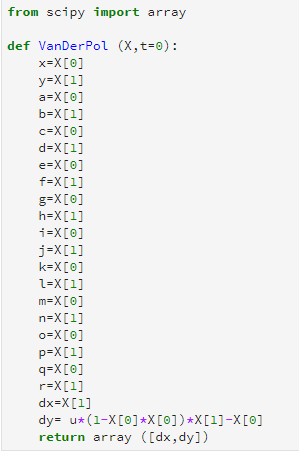
\includegraphics[width=0.25\textwidth]{1.png}
\end{wrapfigure}

Maxima es un software libre, de los más antiguos CAS (Computer Algebra Systems), fue creado en el MIT en la década de los 60, llamado Macsyma en ese entonces, pero adquirió popularidad hasta mediados de los 70. Este software permite resolver cálculos de diferentes áreas de la matemática, desde aritmética hasta ecuaciones diferenciales o incluso gráficos en 2D y 3D.\\

Durante este curso estaremos utilizando wxMaxima, que es una versión simplificada o más amigable para un usuario principiante, 

\section{Infraestructura de Maxima}

En esta sección se presentan algunos conceptos y funciones básicas para entender el funcionamiento y poder utilizar Maxima.

\begin{center}
 
\includegraphics[height=4.5cm]{2.png}
 \end{center}

\subsection{Data I/O}

Cuando se inicia una sesión en Maxima aparece "(\%i1)", que indica la entrada (input) 1, en esa fila se puede escribir un comando y al terminarlo siempre es necesario agregar un punto y coma ";", así se crea una variable interna llamada "(\%i1)", que puede ser llamada posteriormente. Análogamente, el resultado obtenido será en el siguiente renglón con el tag de "(\%o1)", refiriéndose a la salida (output) 1.

\begin{center}
 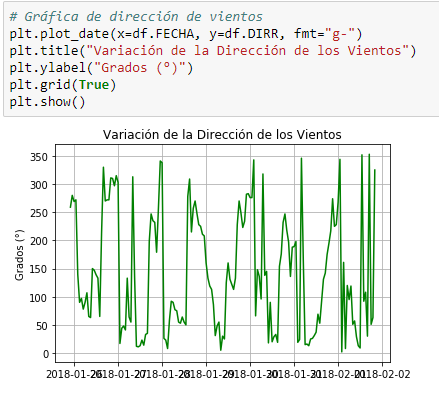
\includegraphics[height=2.5cm]{3.png}
 \end{center}

\subsection{Números, Variables y Constantes}

Maxima acepta números reales (enteros, racionales e irracionales) y complejos. Los números racionales se pueden presentar como fracciones o números de punto flotante. Por su lado, los números irracionales como $\sqrt[]{2}$ o $log(2)$, se presentan en el output de igual manera (sqrt(2), log(2), respectivamente), es decir, no se aproximan, para evitar errores de redondeo, sin embargo, si se desea una aproximación numérica, se puede utilizar la función \textbf{"float"}, que permite convertir a decimal el número ingresado, con una aproximación de 15 a 17 dígitos significativos. Aunque con la función \textbf{"fpprec"} y \textbf{"bfloat"}, se puede ajustar el número de dígitos significativos que se desean\\

También, con la función de \textbf{"rationalize"}, es posible escribir el número en forma fraccionaria, esto permite evitar errores, ya que finalmente, se trabaja con un sistema de computadora que no permite representar ciertos números y tiende a redondearlos. \\

Para asignar el valor a una variable, se utiliza el símbolo ":", ya que "=" se utiliza para ecuaciones. Los caracteres aceptados para nombrar variables son letras, números, \% o \_, con la condición de que el primer caracter no puede ser un número. Los valores asignados a las variables pueden ser números u objetos como expresiones. \\

\begin{center}
 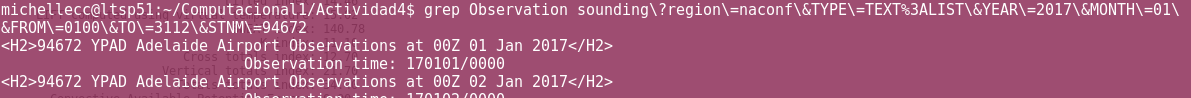
\includegraphics[height=2.5cm]{4.png}
 \end{center}

Para desasignar su valor a la variable se puede utilizar la funcion \textbf{"remvalue"}, para hacerlo para todas, se puede utilizar el comando remvalue(all). A las variables también se les puede asignar una lista de datos, definiéndola de la misma manera, pero utilizando corchetes, ej: a:[1,2,3].\\

\begin{center}
 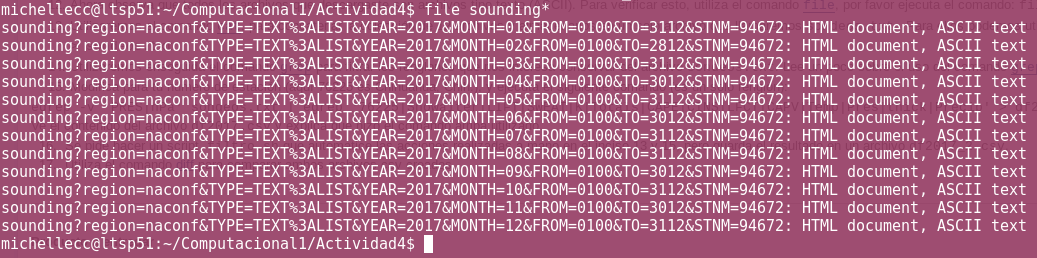
\includegraphics[height=1cm]{5.png}
 \end{center}

Por su parte las constantes son valores predefinidos por Maxima, para llamarlos se utiliza el símbolo \%. Por ejemplo \%pi, \%e, \%i. 

\begin{center}
 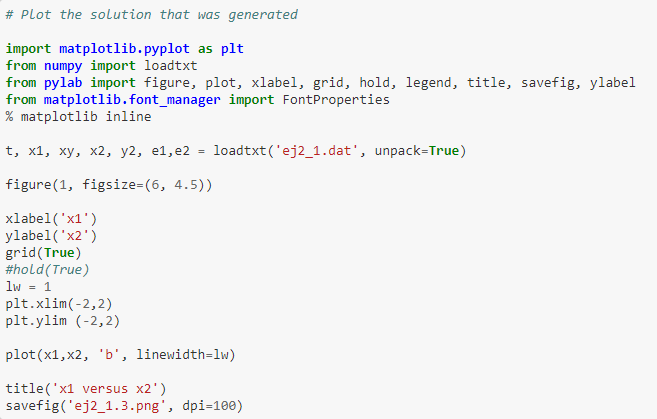
\includegraphics[height=1.5cm]{6.png}
 \end{center}

\subsection{Aritmética}

Los símbolos utilizados para realizar operaciones son: 
\begin{itemize}
\item Suma: +
\item Resta: -
\item Multiplicación: *
\item División: /
\item Exponentes: \^. 
\item Raíz cuadrada: sqrt()
\item Raíz enésima: \^(1/n)
\item Logaritmo natural: log(a)
\item Logaritmo base n de a: log(a)/log(n).
\end{itemize}

\subsection{Plots}

Maxima también permite gráficar en 2D y 3D. 

\subsubsection{Plot en 2D}

Para gráficar en el plano (una variable), se utiliza la función \textbf{"plot2d"}. Es posible gráficar una o varias funciones:

\begin{center}
plot2d([f1(x), f2(x),...,fn(x)], [x,a, b], [png\_file, "archivo.png"). 
\end{center}

El comando anterior permite crear, en una sola imagen, las gráficas de n funciones que dependen de x, donde x irá de a hasta b y se guardará en un archivo png en la carpeta donde se esta corriendo maxima. \\

\begin{center}
 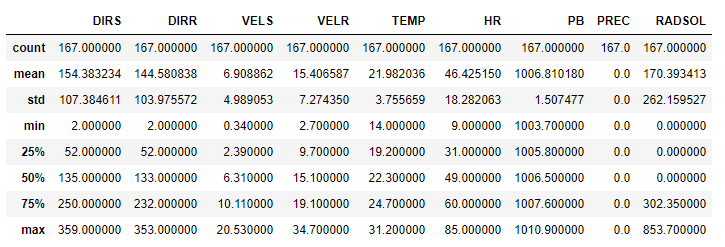
\includegraphics[height=5.5cm]{7.png}
 \end{center}

También es posible graficar puntos: plot2d([discrete, p]). Donde p almacena los puntos a graficar.

\subsubsection{Plot en 3D}

Por otro lado, también es posible graficar funciones que dependan de dos variables, de manera análoga, se utiliza el comando plot3d: 

\begin{center}
plot3d(f(x,y), [x,a,b], [y,c,d])
\end{center} 

\begin{center}
 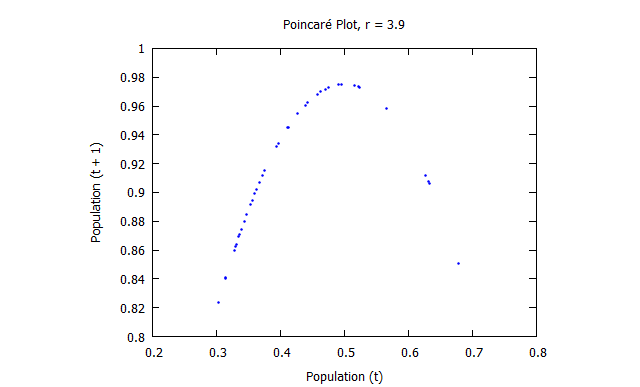
\includegraphics[height=8cm]{8.png}
 \end{center}

\clearpage
\section{Áreas de matemáticas de interés}

En esta sección se presentan posibles comandos o funciones a utilizar en las áreas en las que más trabajo. 

\subsection{Álgebra}

En los renglones de input o output, además de operaciones aritméticas, también se pueden añadir ecuaciones o expresiones algebraicas, utilizando los mismos símbolos mencionados en la sección 2.3.  \\

Para encontrar las raíces de un polinomio se utiliza la función "\textbf{allroots}", donde se pone como argumento el polinomio o la variable que corresponde a este. \\

\begin{center}
 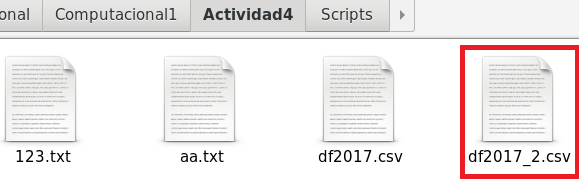
\includegraphics[height=3cm]{9.png}
 \end{center}

Para resolver una ecuación para cierta incógnita, se utiliza la función "\textbf{solve}".\\

\begin{center}
 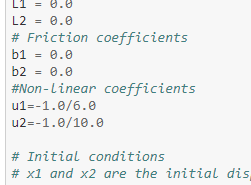
\includegraphics[height=3cm]{10.png}
 \end{center}

Para desarrollar una expresión se utiliza la función "\textbf{expand}" y viceversa, para factorizarla, se utiliza la función "\textbf{factor}".  \\

\begin{center}
 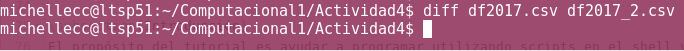
\includegraphics[height=3cm]{11.png}
 \end{center}

\clearpage
La función "\textbf{subst}" sustituirá valores en la ecuación dada. 

\begin{center}
 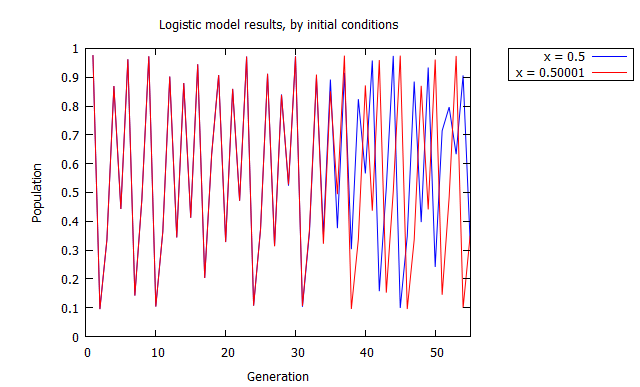
\includegraphics[height=1.5cm]{12.png}
 \end{center}

\subsection{Cálculo}

Para encontrar la derivada de cierta función se utiliza el comando \textbf{diff(f,x)}, donde se calcula la derivada de la función f con respecto a x. \\

\begin{center}
 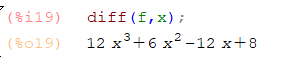
\includegraphics[height=2cm]{13.png}
 \end{center}

De igual manera, para calcular la integral definida de f con respecto a x se utiliza \textbf{integrate(f,x)}.\\

\begin{center}
 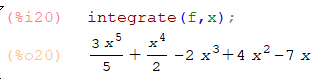
\includegraphics[height=2cm]{14.png}
 \end{center}

Para calcular la integral definida, se utiliza el mismo comando \textbf{integrate(f,x,a,b)}, donde a y b son los límites superior e inferior, respectivamente, de la evaluación\\

\begin{center}
 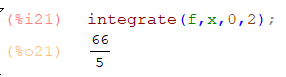
\includegraphics[height=2cm]{15.png}
 \end{center}

Por otro lado, para realizar una integración numérica, se puede utilizar la función \textbf{quad\_qags}. \\

\begin{center}
 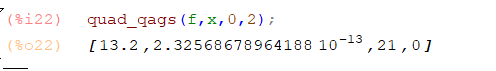
\includegraphics[height=1.5cm]{16.png}
 \end{center}


\section{Ejemplo}

El siguiente ejemplo se tomó del examen parcial 1 de Cálculo IV, del tema Integrales Dobles:\\

Se pretende usar varios modelos de carpas para una celebración (dos de estas se muestran en la figura de abajo). Determine el volumen que encierra cada una de ellas con respecto al suelo, si el techo esta dado por a) $z+y^2=10$ sobre una base cuadrada [-2,2] x [-2,2], b)  $z=6+5e^(-x^2-y^2)$ con sombra $x^2+y^2 \leq 4$, y compare...\\

a) Primeramente se grafica la función: 

\begin{center}
 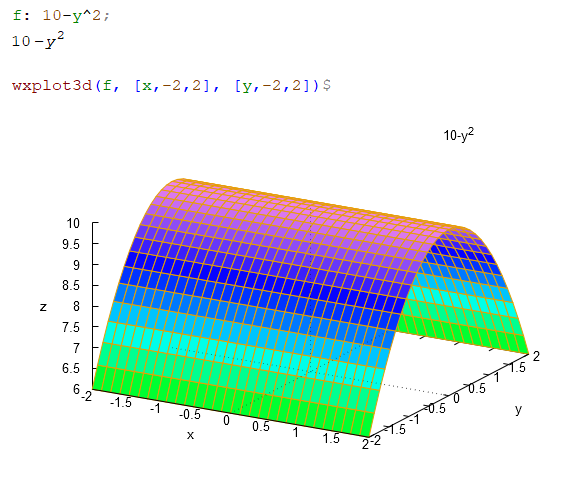
\includegraphics[height=9cm]{17.png}
 \end{center}
 
 Y posteriormente, se realiza la integración de la función.
 
 \begin{center}
 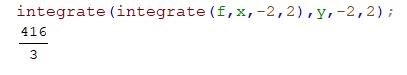
\includegraphics[height=2cm]{18.png}
 \end{center}
 
 b) De igual manera, se realiza la gráfica de la función.: 
 
 \begin{center}
 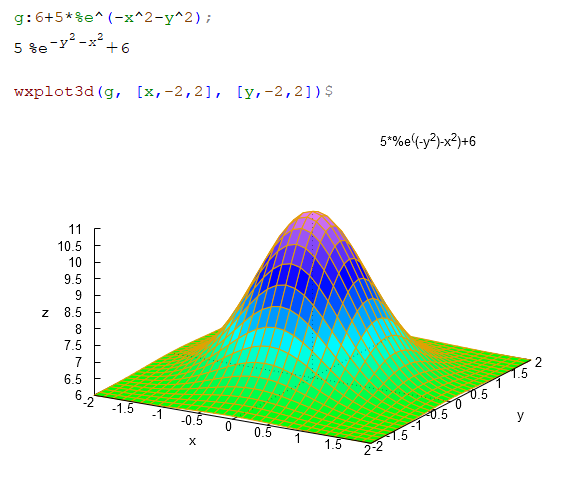
\includegraphics[height=10cm]{19.png}
 \end{center}
 
 Y se integra, pero realizando antes, a mano, un cambio a coordenadas polares: 
 
 \begin{center}
 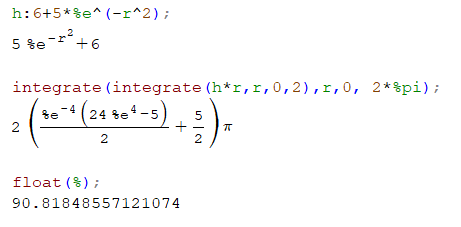
\includegraphics[height=5cm]{20.png}
 \end{center}

Concluyendo que la carpa que abarca más volumen es la del inciso a). 
\section{Diccionario de funciones básicas}

En la siguiente sección se presentan algunas funciones, que se espera sean las más utilizadas: 

\begin{itemize} 
\item coeff(a,b,c): da el coeficiente de b, elevado a la c en la expresión a.
\item cons(a,b): añade a, a la lista b, como el primer elemento.
\item denom(a): da el denominador de a. 
\item desolve(a,b): resuelve un sistema a, de ODE, de b ecuaciones usando transformadas de Laplace.
\item determinant(a): determinante de a. 
\item ident(a): regresa la función de identidad a x a. 
\item imagpart(a): parte imaginaria de a. 
\item integrate(a,b): integral indefinida de a con respecto a b. 
\item invert(a): invierte una matriz. 
\item kill(a): elimina una variable.
\item limit(a,b,c): limite de a, cuando b tiende a c.
\item loadfile(a): carga un archivo en el directorio en el que se encuentra. 
\item matrix(a1,a2,...,an): crea una matriz. 
\item num(a): numerador de a.
\item ode2(a,b,c): resulelve EDO de primero o segundo orden.
\item realpart(a): parte real de a. 
\item taylor(a,b,c,d): serie de Taylor.
\item transpose(a): matriz transpuesta de a.
\item trigsimp(a): simplificación trigonométrica.
\end{itemize}

\section{Conclusiones}
En lo particular, no conocía Maxima y tampoco cuento con softwares como Wolfram o Maple, debido al alto costo, suelo utilizar una plataforma online llamada Symbolab e incluso Geogebra, sin embargo, en ocasiones se encuentra bastante limitado, por lo que el hecho de que se me haya presentado este software libre y muy trabajado, ya que no es nuevo y creo poder explotar su potencial, lo poco que conocí, al nivel de conocimiento que hemos adquirido en programación, me parece ser bastante manejable, útil y confiable. 

\section{Bibliografía}

\begin{itemize}
\item Maxima 5.41.0 Manual (2017). Consultado: 28 de Abril del 2018, de Maxima Source Forge. Sitio web: http://maxima.sourceforge.net/docs/manual/intromax.html\#tth\_sEc8
\item A partial list of Maxima functions(2010). Consultado: 28 de Abril del 2018, de Maxima Source Forge. Sitio web:\\
http://maxima.sourceforge.net/docs/manual/maxima\_singlepage.html\#SEC\_Top
\item Maxima Tutorial (2018). Consultado: 28 de Abril del 2018, de Jaime E. Villate. Sitio web: https://def.fe.up.pt/dynamics/maxima\_tutorial.html
\item Maxima by Example(2009). Consultado: 28 de Abril del 2018, de Edwin L. (Ted) Woollett. Sitio web: \\
http://web.csulb.edu/~woollett/
\end{itemize}

\section{Apéndice}
\begin{enumerate}
\item ¿Cuál fue tu primera impresión de wxmaxima?

Me pareció bastante digerible, fácil de usar, aunque con interfaz algo anticuada o básica.

\item ¿Crees que esta herramienta puede ser útil en otros de tus cursos?

Sí, ya que, como mencioné en las conclusiones, yo si hago uso de la tecnología para resolver problemas matemáticos que se me presentan.

\item ¿Qué se te dificultó mas en esta actividad?

Realmente nada, ya que fue únicamente leer, resumir y entender, así como resaltar funciones importantes.

\item ¿Se te hizo compleja esta actividad? ¿Cómo la mejorarías? 

No, bastante fácil y no la mejoraría porque creo que es necesario empezar a usar un programa con un poco de literatura previa, para poder entender lo básico, incluso recomendaría una actividad así al empezar a trabajar con Python. 

\end{enumerate}


\end{document}